% !TeX spellcheck = it_IT
\documentclass[11pt, twocolumn]{article}

\usepackage{graphicx}
\usepackage{enumitem}

\newenvironment{myitemize}
{ \begin{itemize}[topsep=0ex]
		\setlength{\itemsep}{0pt}
		\setlength{\parskip}{0pt}
		\setlength{\parsep}{0pt}     }
	{ \end{itemize}                  } 

\newenvironment{myenumerate}
{ \begin{enumerate}[topsep=0ex]
		\setlength{\itemsep}{0pt}
		\setlength{\parskip}{0pt}
		\setlength{\parsep}{0pt}     }
	{ \end{enumerate}                  } 


\title{Technological Infrastructures}
\author{}
\date{}

\begin{document}

\maketitle

\begin{abstract}
L'obiettivo del corso è forninre conoscenza solida delle piattaforme tecnologiche e computing platforms.
Differenza delle responsabilità di Data Scientist e Data Engineer.
Il corso è diviso in 2 parti.
L'esame consiste in 15 domande sia aperte che chiuse per parte e si può arrivare a 30 con lo scritto, si può fare un progetto non obbligatorio che vale al più 3 punti.
\end{abstract}

%\section{Lezione 1 - 02/10}

%\section{Lezione 2 - 08/10}

\section{Componenti di NIST}
NIST sviluppa standard di riferimento per il pubblico. Software Architecture è un organizzazione globale di sistemi software, quindi consiste in:
\begin{myitemize}
	\item divisione della componenti software in sottosistemi; 
	\item Definisce le politiche con cui questi sistemi interagiscono;
	\item definisce le interfacce tra le varie componenti.
\end{myitemize}
Un'architettura di riferimento è essenzialmente un template (scatola vuota con elementi prefissati), fornisce solo il vocabolario usato comunemente per discutere le implementazioni di un dato software.\\
Un'architettura di riferimento per il software non è altro che architettura software dove le strutture e i vari elementi e relazioni sono forniti dai template.
\\
NIST fornisce l'architettura di riferimento per i Big Data che:
\begin{myitemize}
	\item Fornisce un linguaggio comune per i stakeholders;
	\item Incoraggia aderenza ai standard comuni;
	\item Permette di implementare le architetture con una certa consistenza;
	\item Illustra e migliora la comprensione delle componenti, processi e  sistemi di Big Data;
\end{myitemize}

\subsection{I 5 ruoli principali per Big Data}
L'architettura concettuale dei Big Data è un architettura a croce con due assi: Information value (IV) e Information Technology (IT) (Fig \ref{fig:NBDRA}).\\
\begin{figure*}
	\centering
	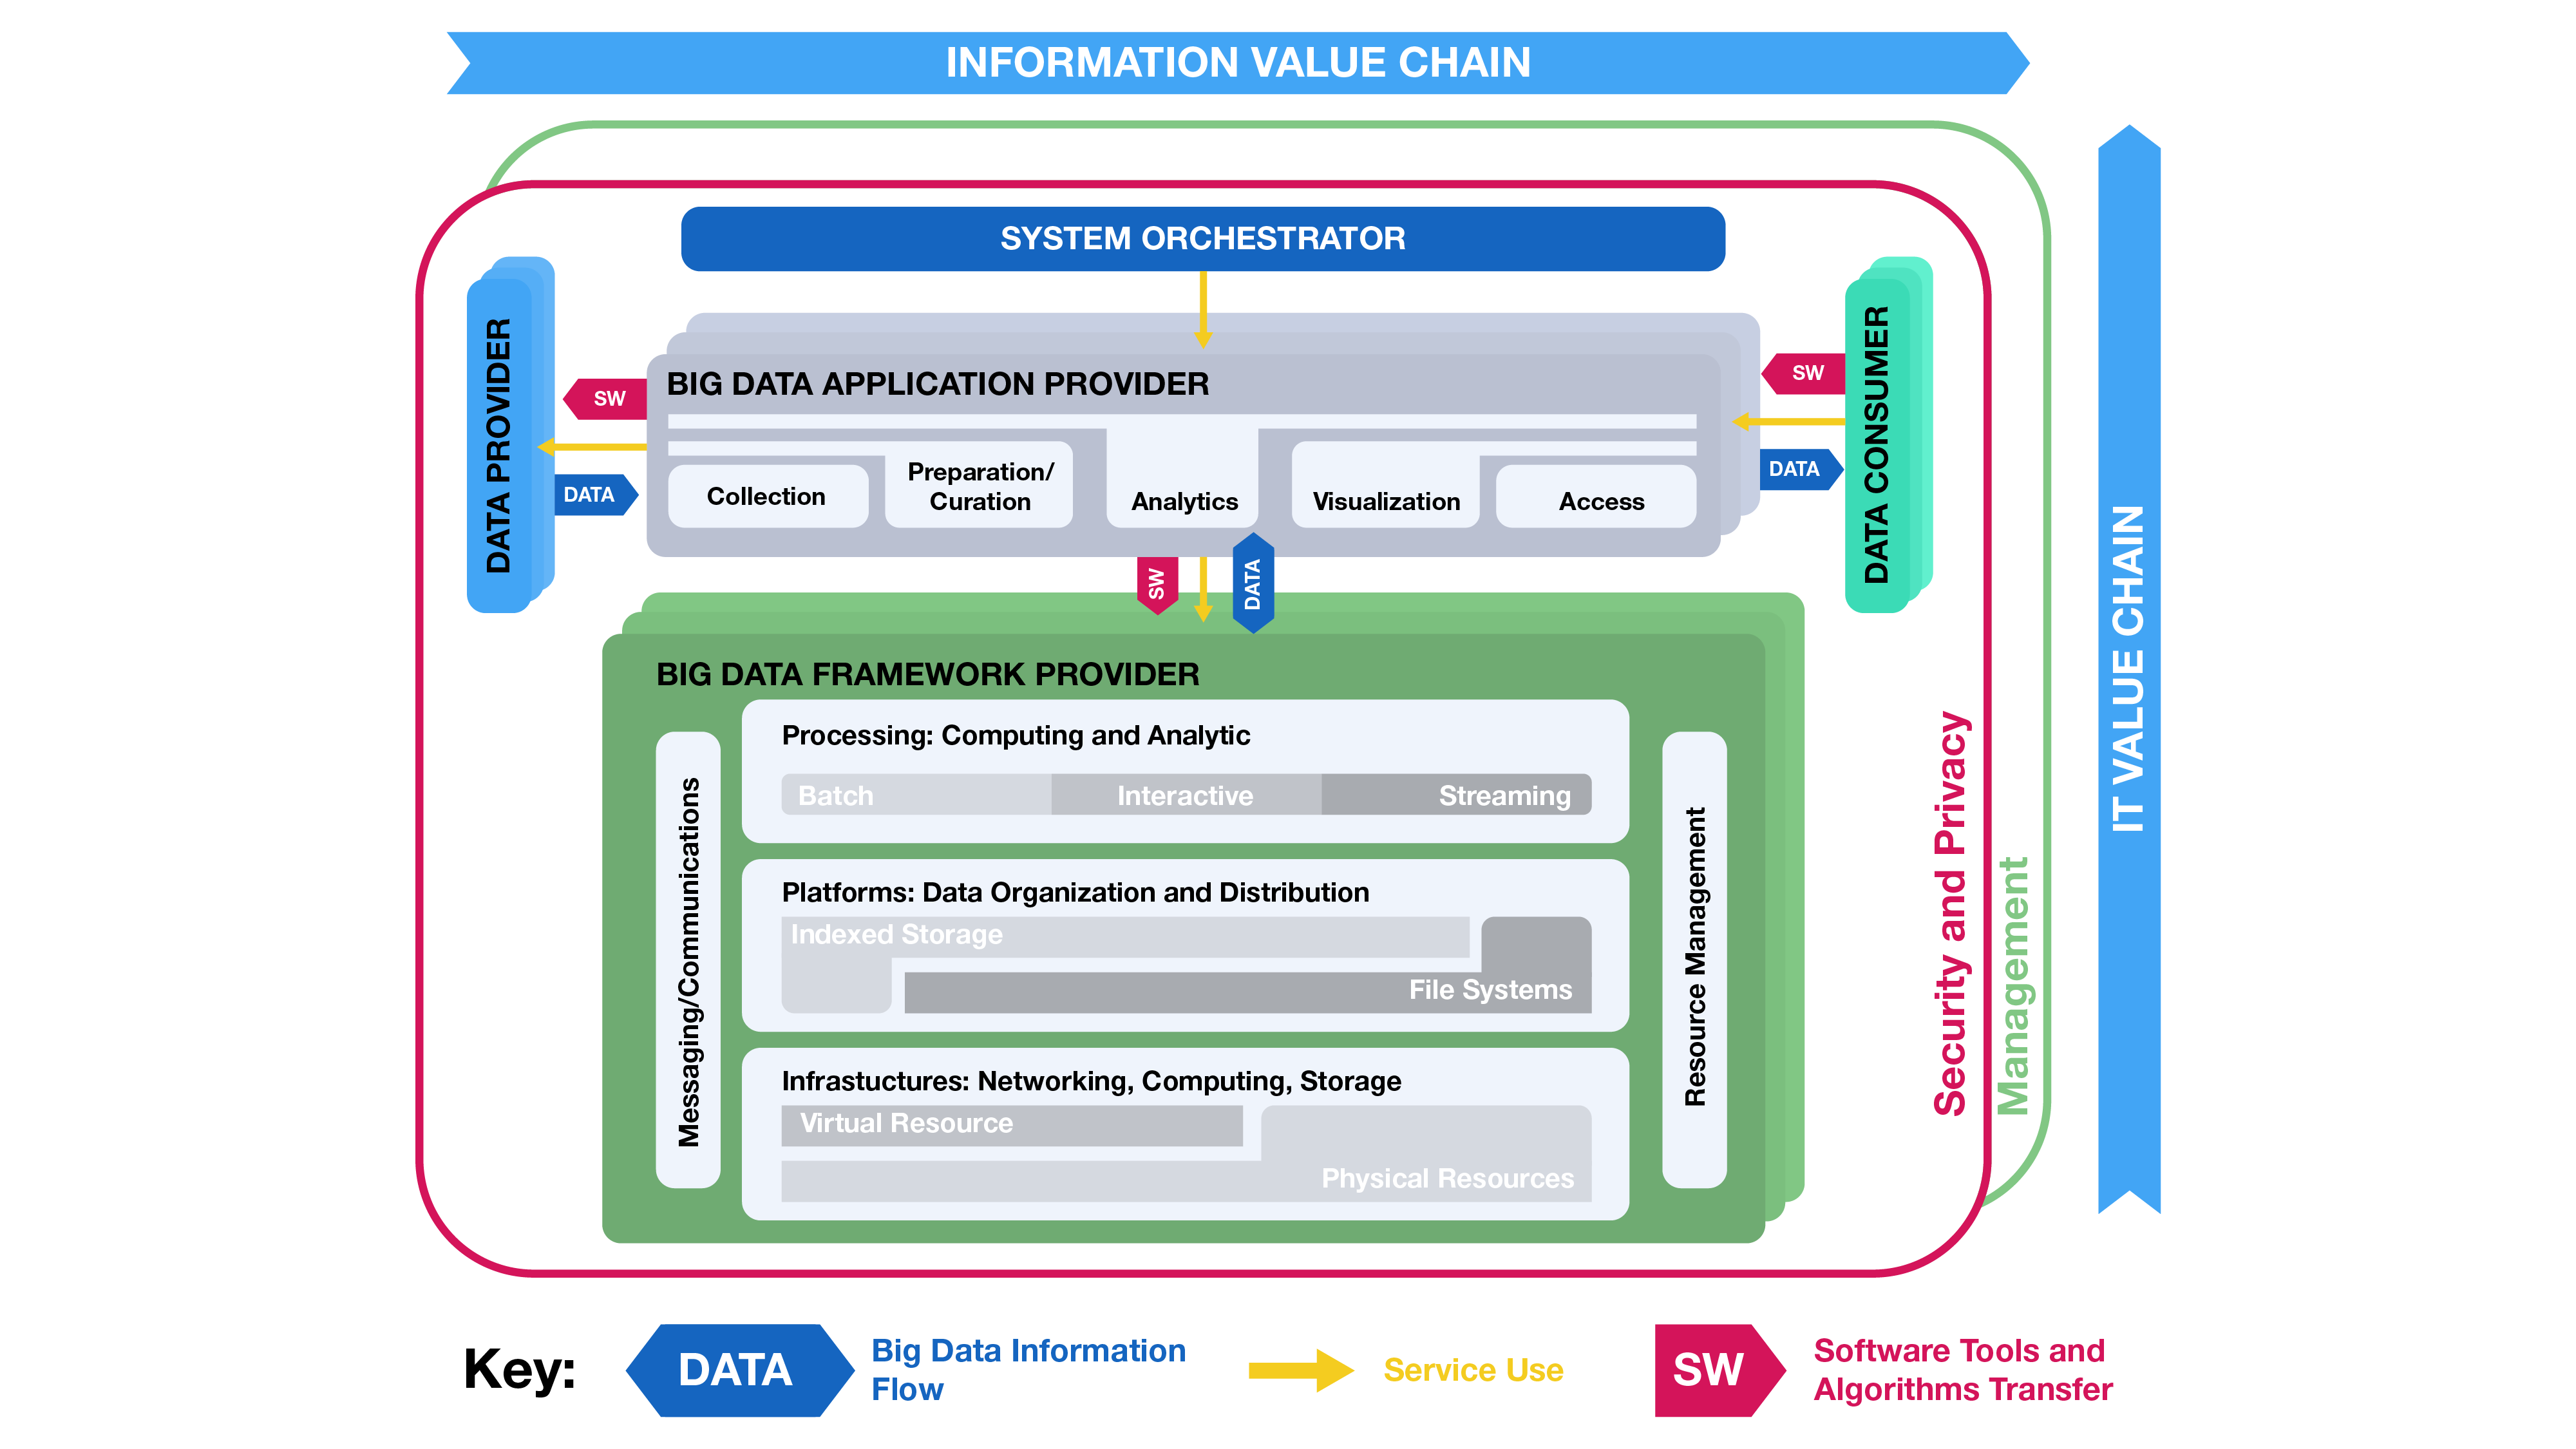
\includegraphics[width=18cm,height=8cm]{imgs/NBDRA_model}
	\caption{NBDRA Conceptual Model}
	\label{fig:NBDRA}
\end{figure*}
I 5 ruoli principali sui 2 assi dei Big Data abbiamo:

\subsubsection{System Orchestrator}
Il system orchestrator coinvolge spesso anche Information Value chain, poiché si preoccupa di implementare e monitorare i processi business a livelli enterprise e le varie politiche sui dati: Redere i dati accessibili per un tempo limitato oppure fornire i dati a velocità diversa(passando il dato in memoria al disco).
Può assegnare/fornire componenti framework fisici o virtuale al sistema, questa assegnazione può essere molto spesso elastica ed indipendente.
Può fornire supporto GUI e collegare i varie applicazioni a un livello alto, e attraverso il management fabbric monitorare i carichi e il sistema per garantire/specificare la qualità del servizio necessaria per i vari carichi.
E' molto spesso centralizzato.
Es. Ambari/Cloudera

\subsubsection{Data Provider}
Può essere sia un software (ad es. in una pipeline più grande) che una persona. Se è una persona metterà i suoi dati e userà gli strumenti di collection e curation/preparation per caricare i dati sul sistemi e migliorarne la qualità, Se un software metterà is suoi dati a disposizione attraverso delle interfacce come Apache Scoop. 
Il data provider può essere interno o esterno alla piattaforma, deve fornisce i diritti di accesso ai dati, ed è obbligato a seguire le policy di privacy e security fabbric. 
I dati possono essere inseriti in pull o push.
es. Flume per caricare i dati da MySQL a HDFS.

\subsubsection{Data Consumer}
Riceve i output dei sistemi BigData, può anche lui fare pull e push dei dati, può usarli le informazioni per data reporting, retrival/search e visualization. Ci deve essere l'autenticazione ed autorizzazione daparte della privacy and security fabbric per la comunicazione tra l'architettura e il Data Consumer.

\subsubsection{Big Data Application Provider}
Corrisponde alle attività tipiche di un Data Scientist, che esistono anche nei sistema tradizionali ma hanno delle trasformazioni nella implementazioni con i Big Data. Queste attività sono:
\begin{myitemize}
	\item Collection: Si occupa di gestire l'interfaccia fornita dal Data Provider, salva/gestisce questi dati in una certa zona affinché questi non vengano persititi, inoltre implementa funzionalità di estrazione dati dal data provider;
	\item Preparation: Effettua Data Validation, rimozione outlier, standardizzazione, formattazione e arricchimento. 
	Cerca di promuovere dati di alta qualità;
	\item Analytics: Estrazione conoscenza dai dati, sfruttando il software sottostante del Big Data Framework Provider;
	\item Visualization: Presentazione dati in maniera visuale;
	\item Access: E' l'opposto della collection, si preoccupa di esporre i dati verso l'esterno. 
\end{myitemize}

\subsubsection{Big Data Framework Provider}
Fornisce le infrastrutture per supportare i Big Data Application Provider. Si occupa in particolare di:
\begin{myitemize}
	\item Processing dei dati - ha una dualità: da una parte è un framework che mette a disposizione delle interfacce per la programmazione per fare certe cose (es. MapReduce) e dall'altra parte definisce come l'implementazione viene effettuata. I framework possono variare tra un proccessamento batch e in streaming.
	\item Platforms per l'organizzazione e immagazzinamento dei dati - può contenere i meta-dati insieme alle descrizione semantiche dei dati. 
	Può essere relazionale distribuito o non relazionale.
	\item Infrastructures per l'esecuzione fisica del nostro software, è l'insieme delle risorse computazionali fisiche o virtuali sulle quali il nostro sistema Big Data gira, può essere costituito da server di grandi o piccole dimensione. 
	Queste componenti forniscono:
	\begin{myitemize}
		\item Networking - Possono essere definiti attraverso software e possono essere reti fisiche che può essere a sua volta partizionato in reti virtuali. 
		Possono essere reti puramente virtualizzate cioè tutto quanto (firewall, router, load balancing) sono realizzate in maniera virtuale (es. VM dentro la nostra macchine);
		\item Computing - Hardware, Software, OS, memoria per il computing;
		\item Storage - dischi per storare (in locale), RAID, in rete ecc.
		\item e altri servizi come il Raffrendamento, l'apparto elettrico e la sicurezza
	\end{myitemize}
	Può essere deployato su ambienti fisici che virtualizzati (nativi, hostati o contenerizzati).
\end{myitemize}
Inoltre ha 2 ruoli diffusi nelle 3 componenti sopraindicate:
\begin{myitemize}
	\item Comunicazione e messaggistica tra le componenti;
	\item Gestione delle risorse per l'integrazione delle componenti.
\end{myitemize}

\subsection{I 2 ruoli diffusi per Big Data}
questi 2 ruoli prendono il nome di Fabric, il termine Fabric(tessuto) viene usato perché queste 2 ruoli cross-cutting, cioè sono presenti un pò ovunque nell'architettura.

\subsubsection{Management fabbric}
Le due attività principali associate:
\begin{myitemize}
	\item Gestione del sistema per provvedere le risorse, gestione dei software e pacchetti e infine la gestione delle configurazioni e performance delle varie pipeline;
	\item Ciclo di vita dei Big Data, BDLM (Big Data Life Cycle Management), contiene l'enforcing delle Policy (es. encoding/decoding), gestione dei meta data (data governance), accessibilità dei dati, data recovery e la loro preservazione.
\end{myitemize}


\subsubsection{Security and Privacy Fabric}
Si occupa delle tre caratteristiche tipiche delle security: 
\begin{myitemize}
	\item Autenticazione: Indica tutte le attività che validano l'utente;
	\item Autorizzazione: Una volta autenticato l'utente verifica i suoi permessi, es. alcuni dati potrebbero non essere accessibili a certi utenti;
	\item Auditing: riguarda la registrazione degli eventi che accadono nel sistema, può far partire un allarme in caso di evento anomalo o a posteriori analizzare la sequenza di eventi (con i file log).
\end{myitemize}

\section{Virtualizzazione}
Per i computer sono stati definiti con le 5 componenti classiche:
\begin{myenumerate}
	\item Input Devices: Tastiera ecc.
	\item Output Devices: Display ecc.
	\item Storage Devices: Volatile(RAM), Permanente(HD, SSD)
	\item Processore:
	\begin{myitemize}
		\item Datapath
		\item Control
	\end{myitemize}
	\item Network
\end{myenumerate}
La virtualizzazione permette l'esecuzione di più sistemi operativi simultaneamente sulla macchina in maniera totalmente isolata. 
Può essere visto come una emulazione di un software o hardware su cui altri software possono eseguirsi, questo ambiente emulato è detto virtual machine.
Il concetto di VM è stato sviluppato negli anni 60 da IBM sui mainframes.
Viene abbandonato con la nascita di PC moderni e ripreso con la crescita recente di cloud. La virtual machine viene ottenuto attraverso un Virtual Machine Monitor detto anche ipervisore.\\
L'\textbf{Hypervisor}(Ipervisore) è un software che giace sotto gli OS virtualizzati per offrire le funzionalità di condivisione delle risorse disponibili in modo tale che il programma o OS in esecuzione veda queste risorse come se fosse a lui dedicate. 
Le risorse sono CPU, memoria, storage e la rete.\\
Vi sono diversi benefici della virtualizzazione:
\begin{myitemize}
	\item Visione unificata delle risorse es. vedo tanti dischi come un unico disco;
	\item Consolidazione delle risorse virtualizzate, in modo da avere l'ottimo utilizzo delle risorse;
	\item Facilità di implementare la ridondanza per copiare gli ambienti virtualizzati;
	\item Facilità la migrazioni di sistema su un altro, inoltre se non cambio ipervisore la macchina(virtuale) funzionerà identicamente a prima;
	\item Gestione centralizzata del hardware e software.
\end{myitemize}
Altri benefici/proprietà della virtualizzazione sono:\\
\textbf{Workload Isolation:} attraverso la virtualizzazione è possibile isolare completamente i programmi, che ha miglioramenti anche nella sicurezza, inoltre aumenta affidabilità poiché il fallimento di un programma non comporta fallimento dei programmi poiché sono isolati, inoltre si risolvono anche i problemi riguardanti i conflitti di librerie in questo modo. Infine si ottiene un controllo sulle performance poiché l'esecuzione di una VM non affligge il performance dell'altra;\\
\textbf{Workload Migration:} ciò aiuta in:
\begin{myitemize}
	\item Mantenimento di Hardware;
	\item Load Balancing;
	\item Fault Tolerance;
	\item Disaster Recovery.
\end{myitemize}
Poiché possiamo spostare tutto l'ambiente virtualizzato su una nuova macchina in maniera abbastanza trasparente, per fare ciò la macchina dovrebbe essere sospesa, totalmente serializzata per essere inviata nella rete, migrata su una nuova macchina e fatta ripartire immediatamente o solo salvata senza esecuzione.\\
\textbf{Consolidazione:} Sfruttando il Workload Migration è possibile consolidare macchine separate su un unica piattaforma riducendo i costi (usata molto spesso nei Datacenter in orari non di picchi).\\
\begin{figure}[h]
	\centering
	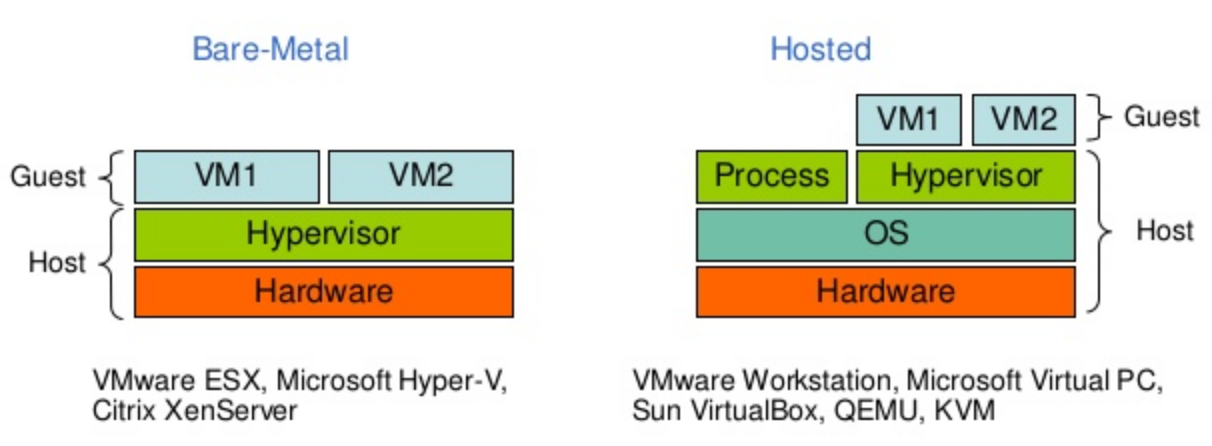
\includegraphics[width=\linewidth]{imgs/hypervisor_type.png}
	\caption{I tipi di Hypervisor}
	\label{fig:hypervisor_type}
\end{figure}
I diversi tipi di HyperVisor sono (Fig \ref{fig:hypervisor_type}):
\begin{myitemize}
	\item \textbf{Hosted}: in questo caso ipervisore è un processo che gira al di sopra del sistema operativo e permette l'esecuzione di più macchine Guest.
	In questo caso quindi bisogna installa prima un OS su cui verrà installa VMM (ipervisore) e adesso l'host potrà eseguire le applicazioni all'interno della sua finestra.
	Il vantaggio qua è la facilità di installazione e configurazione, inoltre la HostOS e GuestOS sono non modificati e non dipendono dal particolare hardware, ma gli svantaggi sono la degradazione delle performance e la mancanza di supporto real time OS poiché vi sono varie entità/software in mezzo;
	\item \textbf{Bare-Metal}: in questo caso ipervisore funziona direttamente al di sopra del Hardware.
	In questo caso l'ipervisore è un OS molto leggero e comunica direttamente con hardware al posto di dipendere su un altro OS. 
	I vantaggi sono miglioramento in I/O e supporto real time, mentre gli svantaggi sono la difficoltà di istallazione e configurazione e la dipendenza dal tipo di hardware specifico.
\end{myitemize}
Ci sono principalmente 2 tecniche di virtualizzazione: \textbf{Software Virtualization} (di cui abbiamo parlato fino ad adesso) e \textbf{Hardware Assisted Virtualization}.\\
Nella \textbf{Virtualizzazione Totale} VMM si preoccupa di emulare in maniera completa tutto l'hardware, quindi avremo un processore, memoria, disco e network virtuale.
in questo caso OS ospite non è consapevole dell'esistenza dell'ambiente virtuale e ogni macchina è del tutto indipendente.
A livello CPU, avviene la traduzione binaria: Questo avviene in diversi anelli di sicurezza, in particolare sono 4, dove l'anello 0 è quello più privilegiato e permette l'esecuzione del codice direttamente sul hardware e qua dove viene eseguito il kernel dell'OS.
Le applicazione dell'utente vengono eseguite sull'ultimo anello (anello 3).\\
L'ipervisore gira sull'anello 0 mentre le GuestOS gira sull'anello 1, quindi hanno più permessi delle normali applicazioni. 
VMM ha accesso sul anello 0 per avere accesso diretto sulla CPU piuttosto che virtualizzarla. \\
La \textbf{Para-Virtualizzazione} ha un approccio diverso rispetto alla virtualizzazione totale (è una via di mezzo tra total virtualization e bare-metal), in questo caso il Guest sono consapevoli della VMM e usa chiamate speciali in alcuni casi per essere eseguite direttamente sul hardware e ciò comporta un miglioramento nella performance ma ciò lo rende meno flessibile.\\
La \textbf{OS-level Virtualization (Containerization)} non usa la VMM, la virtualizzazione è fornita direttamente dal HostOS che esegue tutte le funzioni di un ipervisore totalmente virtualizzato, quindi ha una partizione puramente virtuale delle risorse, e ciò comporta un'assegnazione flessibile delle risorse alle varie applicazioni. Es. Docker.\\
Ci sono 3 modelli di servizio:
\begin{myenumerate}
	\item \textbf{Server Virtualization}: supponiamo di avere diversi server su macchine diverse, in caso di un problema (crash di un nodo) o vi è un bisogno di upgrade, in caso di macchine fisiche dovrò prendere lo stesso modello o lo stesso vendore, la soluzione è quella di sfruttare una medesima macchina con un virtualizzatore e mettere i diversi server insieme.
	In questo modo ho una consolidazione, risorse condivise, una gestione centralizzata, facilità di migrazione, maggiore ROI e meno spazio occupato.
	La Disaster Ricovery e scalabilità viene facilitata, diversi modelli a scelta (basta che sia uguale l'ipervisore), ho maggiore disponibilità.
	\item \textbf{Desktop Virtualization}: è la tecnologia che separa l'ambiente desktop e le applicazione software dal cliente fisico che lo usa. 
	Il nostro desktop diventa un thin client che usa PC privo della memoria RAM e potenza calcolo necessaria per far funzionare una macchina reale, la macchina gira su un pool di VM su un server su un data center.\\
	I benefici sono molteplici: Upgrade di software e OS facilitato, alta disponibilità, fault tolerance, accessibile da LAN, WAN, Internet, inoltre vi è la possibilità di far eseguire una piccola parte della computazione dal dispositivo locale.
	\item \textbf{Application Virtualization}: Molto simile alla Desktop virtualizzazione, solo che al posto di tutto il desktop, sono le applicazione ad essere in virtualizzate, quindi un applicazione che gira sul desktop, fa la computazione sul cloud, una piccola parte della computazione può essere effettuata anche in locale.
	I vantaggi sono molto simili a quelli del Desktop Virtualization, un vantaggio aggiuntivo può essere che pago solo quello che uso, riducendo i costi delle licenze.
\end{myenumerate}
%\section{Lezione 3 - 09/10}

\section{Cloud}
Definizione ``vera'' del cloud da ricordare: è un tipo di servizio distribuito di sistemi interconnessi e computer virtualizzati dinamicamente provvisionati e presentati come un unica risorsa computazionale basato su service-level agreement.
\\
Sostanzialmente il cloud è la possibilità di avere accesso alle risorse computazionale attraverso la rete on-demand ed è composto da 5 punti chiave, 3 modelli di servizio e 4 modelli di deployement.

\subsection{The 5 Properties of cloud}
Le 5 proprietà aggirano attorno ad una idea centrale del cloud: Utility Computing, SOA (Service Oriented Architecture) + SLA(Service Level Agrement).\\
\textbf{Utility Computing} nel senso che il service provider fornisce le risorse computazionali e le infrastrutture che servono al cliente e li fa pagare in base all'utilizzo piuttosto che con un costo fisso, come i servizi on-demand per massimizzare l'uso efficiente, minimizzando i costi nella maniera meno trasparente possibile(Senza mostrare al cliente tutto ciò che si fa).\\
\textbf{SOA (Service Oriented Architecture)}: è un insieme di servizio che comunicano tra di loro poiché non basta di solito un solo servizio per implementare un servizio web completo per utente.\\
\textbf{SLA (Service Level Agreement)}: è un contratto tra il service provider e il cliente che specifica il livello di servizio che il service provider deve fornire in termini di QoS.
Il \textbf{QoS}(Quality of Service) è un set di tecnologie per gestire il traffico della rete in modo da migliorare la user experience, ormai è associato a un significato più generico riguardante le valutazioni di tecnologie non funzionali, cioè non mi interessa solo la funzionalità (il risultato della mia richiesta) ma anche la sua efficienza.\\
Le metriche più comuni delle SLA sono up-time e down-time, Response time. Se le metriche garantite non vengono rispettato vi sono delle penalità sui service provider.\\
La tecnologia grazie al quale cloud funziona sono:
\begin{myitemize}
	\item Hardware Virtualization;
	\item Computing distribuito e parallelo;
	\item Service-oriented Computing;
	\item Autonomic Computing (reazione a cambiamenti del sistema).
\end{myitemize}

Le 5 \textbf{proprietà/caratteristiche} che identificano il cloud sono:
\begin{enumerate}[noitemsep, topsep=0ex, leftmargin=*]
	\item \textbf{Scalabilità, Elasticità}:
	\begin{itemize}[noitemsep, topsep=0ex, leftmargin=*]
		\item Scalabilità è una proprietà del sistema di crescere in maniera graduale col crescere di richieste, può essere orizzontale (Scale In \& Scale Out) o verticale (Scale Up \& Scale Down).
		\item Elasticità è l'abilità di adattarsi automaticamente per inizializzare la scalabilità.
	\end{itemize}
	Ciò si può ottenere attraverso provisioning dinamico, che fa riferimento è un ambiente complesso che permette la allocazione e de-allocazione on-demand delle istanze/risorse attraverso applicazione o un console amministrativo. 
	Di solito vengono messe delle regole per automatizzare il provisioning, ottenendo così un abbassamento dei costi e performance migliorata.
	
	\item \textbf{Disponibilità, Affidabilità}:
	\begin{itemize}[noitemsep, topsep=0ex, leftmargin=*]
		\item Availibility è il rapporto tra il up-time e tempo totale di esecuzione;
		\item Affidabilità è la capacità di funzionare in situazioni particolari (rottura di un nodo, attacco di hacker) per un certo tempo.
	\end{itemize}
	Questi punti possono essere ottenuti attraverso sistemi di:
	\begin{itemize}[noitemsep, topsep=0ex, leftmargin=*]
		\item Fault Tolerance è la capacità del sistema di continuare ad funzionare anche dopo un fallimento di uno dei suoi componenti, spesso il servizio viene degradato proporzionalmente alla gravità del fallimento ma il servizio continua ad funzionare.\\
		Le caratteristiche principali sono che non ha un singolo punto di fallimento, la componente fallita viene individuata ed isolata per prevenire la propagazione del fallimento;
		\item Resilience è l'abilità di offrire e mantenere un livello di servizio accettabile anche dopo un fallimento, essenzialmente ritornare allo stato di funzionamento dopo un caso di fallimento del sistema (ad es. viene a mancare l'elettricità).
		Quindi i sistemi devono avere le policy e procedure per il recupero, ad es. Backup (dei dati off-site oppure di tutto il sistema) oppure preparazione contro fault come un una corrente non-interrompibile (UPS) oppure sbalzi di corrente/tensione.
		\item Sicurezza
		La sicurezza riguarda l'impiego di politiche e tecnologie e sistemi di controllo per protegge applicazioni e infrastrutture da accessi malevoli, quindi abbiamo il suo impiego in:
		\begin{itemize}[noitemsep, topsep=0ex, leftmargin=*]
			\item la protezione i dati, mantenendo l'accesso ai dati riservato solo in base ai privilegi;
			\item Gestione dell'identità per garantire l'accesso alle risorse in base ai loro privilegi (protezione dei dati);
			\item Sicurezza dell'applicazione riguarda la possibilità di blindare le nostre applicazioni per accessi malintenzionati;
			\item Privacy per oscurare i dati in base alle leggi privacy e gestiti solo da utenti competenti.
		\end{itemize}
	\end{itemize}

	\item \textbf{Gestibilità, Interoperabilità}:
	La Gestbilità riguarda la gestione di questi sistemi attraverso un singolo punto di accesso mentre la interoperabilità è una proprietà di un prodotto o sistema per lavorare con altri prodotti/sistemi.
	Lo si ottiene attraverso \textbf{System control automation} e \textbf{System State Monitoring} che è un processo che monitora lo stati dei hardware, metriche dei performance, i log dei sistemi, il pattern dei accessi alla rete ecc.
	E' anche collegato al sistema di Billing, poiché gli utenti pagano ciò che usano e il cloud provider deve registrare le risorse/servizio usate da ciascun utente.\\
	\item \textbf{Accessibilità, Portabilità}
	
	\item \textbf{Ottimizzazione, Performance}
	Il \textbf{Load Balancing} è una tecnica per la distribuzione del workload su un sistema di più computer, CPU, HD ecc. per ottenere l'utilizzo ottimale, migliorando così: l'utilizzo del sistema, la performance e l'efficienza energetica riducendo overload.\\
	Il \textbf{Job Scheduler} è un applicazione che ha il compito di eseguire i processi in background (chiamati anche processi batch).
	Nel cloud i task intensivi computazionalmente o task che crescono dinamicamente vanno pianificato con Job Scheduler.
\end{enumerate}
Da un punto di vista dell'utente, lui non vuole sapere come e cosa viene fatto né chi gestisce il servizio, ma vuole solo un servizio funzionale.

\subsection{The 3 Service Model of cloud}
Iniziamo con i tre modelli del servizio del cloud sono:
\begin{enumerate}[wide, topsep=0ex, noitemsep]
	\item \textbf{IaaS (Infrastructure as a Service)}: es. le macchine virtuali, in questo caso il provider/vendor gestisce la virtualizzazione, il cliente ottiene le risorse virtuali, di solito da un catalogo che contiene le specifiche hardware (virtualizzato) pre-selezionate dal provider. Nella maggior parte dei casi gli OS sono anche prefissate per questioni di prestazioni/stabilità e compatibilità con hypervisor da loro usato.
	\item \textbf{PaaS (Platform as a Service)}: ci viene fornito una scatoletta dove scrivere e eseguire/testare le applicazioni, il provider sarà il garante del fatto che il sistema sia abbastanza responsive e abbia un runtime sufficiente. E' meno flessibile rispetto allo IaaS ma allo stesso momento lo sviluppato perde meno tempo nella configurazione delle macchine.
	\item \textbf{SaaS (Software as a Service)}: es. GMail quindi utente non può fare niente tranne usare il software.
\end{enumerate}

In realtà il cloud vero è un po' più offuscato di quanto detto sopra, spesso non è facile collocare il modello di cloud di un'azienda esattamente in uno dei 3 modelli.\\
Un aspetto molto importante da considerare è quello economico, cioè grazie al modello pay-as-you-go cloud il costo capitale (CAPEX) si trasforma in costo operazionale (OPEX), inoltre il rischio di errore nella scegliere le macchine sparisce, se ho bisogno di più potenza richiedo una macchina più forte e se ho bisogno di meno potenza abbasso la potenza e risparmio.
Allo stesso momento i cloud service provider hanno diversi benefici: profitto sfruttando l'economia di scala (comprare un servo costa X, ma comprare N server non costa N*X), possono capitalizzare sui loro investimenti (amazon che vende la potenza residua) o possono sfruttarlo per promuovere un loro prodotto (es. per far usare .NET ai sviluppatori).

\subsubsection{IaaS}
IaaS fornisce automaticamente il processing, storage, network e altre risorse fondamentale per il computing, e l'utente può installare i software che sono per lui necessari.\\
Lo IaaS supporta queste 3 caratteristiche del cloud:
\begin{myitemize}
	\item Gestibilità e Interoperabilità: Attraverso un interfaccia può gestire tutte le VM che vuole, le può pagare come vuole;
	\item Disponibilità ed Affidabilità: gestita dal cloud provider attraverso le zone di disponibilità;
	\item Scalabilità ed elasticità: Proprietà del sistema ma deve essere implementato dall'utente.
\end{myitemize}
L'architettura è composta dall'hardware seguita da un layer di virtualizzazione e l'utente ha accesso a due interfacce:
\begin{myitemize}
	\item Interfaccia per gestione delle risorse, queste risorse sono:
	\begin{myitemize}
		\item VM: creazione, cancellazione, gestione, sospensione delle VM 
		\item Virtual Storage: Allocare spazio, ridurre/aumentare del DB, scegliere servizi con velocità di lettura/scrittura diversi (per prezzo);
		\item Virtual Network: gestione delle IP associate alle VM, registrazioni al dominio delle IP, scegliere la larghezza di banda.
	\end{myitemize}
	\item Interfaccia del il monitoring del sistema: viene messa a disposizione da VIM: L'orchestrazione delle macchine/risorse, in maniera rapida e dinamica, su un server viene gestita dalla Virtual Infrastructure Mangaser(VIM), diverse metriche vengono usate per il monitoraggio es:
	\begin{myitemize}
		\item VM: CPU usage, memory usage;
		\item Virtual Storage: utilizzo del disco, livello di duplicazione dei dati e velocità di accesso al disco;
		\item Virtual Network: L'uso della banda, lo stato di connettività e il bilanciamento sulla rete.
	\end{myitemize}
\end{myitemize}


\subsubsection{PaaS}
PaaS mette a disposizione all'utente i linguaggi di programmazione e i tools (come IDE) supportati dal provider, quindi il controllo sul deployement dell'applicazione è in mani del consumer ma il controllo sulle infrastrutture sottostante è gestita dal cloud provider.
\\
Alla base vi è una archittettura come quella di IaaS, vengono aggiunti i Runtime Environment e sopra questi ci sono i Programming IDE e le API/tools supportati dall'ambiente, spesso hanno in comune le funzioni come: computation e lo storage.\\
Il Runtime Environment si riferisce a una collezione di software, implementati con una collezione di librerie, le proprietà fornite dal Runtime Environment sono:
\begin{myitemize}
	\item Gestibilità ed Interoperabilità
	\item Performance ed Ottimizzazione
	\item Disponibilità ed Affidabilità
	\item Scalabilità ed Elasticità
\end{myitemize}
L'interfaccia messa a disposizione per il controllo del sistema mette a disposizione un set di azioni in base a:
\begin{itemize}
	\item Policy based control: le azioni seguono delle regole per prendere delle decisioni quindi azioni seguite con if <> then <>
	\item Controllo del workflow: descrizione del flusso di installazione e configurazione delle risorse oppure dei daemon.
\end{itemize}

\subsubsection{SaaS}
SaaS: vengono fornite al cliente applicazione del provider in cloud, l'utente non può gestire o sviluppare l'applicazione o gestire l'architetture nel cloud ma può interagire con esso attraverso interfacce ad es. portali/applicazioni web, che con introduzione del Web 2.0 ha potenziato l'iterabilità con l'applicazione in cloud, es: Facebook(Messenger), Office, Skype, DropBox, sistema CRM, sistema medico nazionale, sistema di trasporto pubblico.\\
Il punto fondamentale di questo tipo di cloud è l'Accessibilità e la portabilità.\\
Oss: La differenza tra il portale web e una pagina web è che il portale permette l'integrazione di diverse pagine attraverso dei login.

\subsection{The 4 Cloud Deployement Models}
I 4 modelli primari che differenziano un cloud, basati sulle possibilità di accesso, la dimensione e la proprietà dei servizi, sono:
\begin{myitemize}
	\item \textbf{Public Cloud} (o multi-tenant o external cloud): 
	L'infrastruttura viene messa a disposizione del pubblico generale o almeno alle organizzazioni grandi attraverso pagamento per il suo uso, le caratteristiche sono:
	\begin{myitemize}
		\item Infrastruttura omogenea per garantire le medesime prestazioni a due utenti che pur trovandosi in posti diversi usano lo stesso servizio;
		\item Policy comuni;
		\item Risorse condivise;
		\item Infrastrutture viene affittata;
		\item Economia di Scala.
	\end{myitemize} 
	
	\item \textbf{Private Cloud:} (o on-premise cloud o internal cloud)
	Viene operato da un'unica organizzazione e può essere gestita dalla stessa o un'altra organizzazione, cioè la categoria di utenti è limitata. A differenza del public cloud le caratteristiche sono:
	\begin{myitemize}
		\item Infrastruttura eterogenea per via del costo e dal fatto che una azienda privata non butta via un hardware solo per averli omogeneità;
		\item Policy customizzate ad-hoc per gli utenti;
		\item Risorse dedicate;
		\item Infrastrutture gestita da house;
		\item End-to-end control sui processi.
	\end{myitemize}
	
	\item \textbf{Community Cloud:} è una struttura gestita da diverse entità, in pratica più entità mettono insieme i loro cloud privati per generare un super cloud, ad esempio alcune università americane possono unire i loro cloud per qualche ricerca specifica ecc.
	
	\item \textbf{Hybrid Cloud:} è la comoposizioni di più tipi di cloud, ad esempio un azienda privata crea il suo cloud privato per la gestione di informazioni sensibili e usa il cloud pubblico per il resto, oppure lo usa per la scalabilità in caso di traffico aumentato.
\end{myitemize}

\section{Amazon ECOSYSTEM-IaaS}
Amazon Web Service sono creati per lavorare indipendentemente ma possono interagire tra di loro, condividendo tra di loro le stesse convenzioni di nomi e autenticazione e minimizzando le connessioni interne.
\\
Amazon mette a disposizione il concetto di regione e di zona di disponibilità:
\begin{itemize}[noitemsep, topsep=0ex, wide]
	\item Ciascuna \textbf{Availibility Zone} è un data center indipendente con la propria griglia di potenza e connessione della rete, le zone all'interno di una regione sono collegate tra di loro attraverso connessione a latenza bassa. 
	Il nome deriva dal fatto che sono zone ad alta disponibilità, quindi se una zona fallisce il suo effetto non viene notato dalle altre zone creando così una stabilità ed alta fault tolerance.
	\item \textbf{Regione} è un cluster di Availibility Zone localizzati in una area geografica. 
	Quando si crea una istanza Amazon ci dà la possibilità di scegliere una availability zone (o di default lo si lascia far scegliere ad Amazon) e all'interno della stesso regione è possibile distribuire la propria istanza su più availability zone, quindi se una zona fallisce l'altra (molto probabilmente) continua a funzionare.
	Amazon non fa pagare i trasferimenti di dati all'interno della stessa regione, ma tra regioni le comunicazioni vengono fatte pagare.
\end{itemize}
Esiste AWS GovCloud che è una regione AWS isolata e permette di gestire dati estremamente sensibili e può essere acceduta solo da cittadini Americani verificate dal governo Americano e sul suolo Americano.\\
Uno dei servizi principali di AWS è \textbf{Simple Storage Service (S3)}, un storage object che è un sistema di archiviazione piatto cioè non è possibile creare cartelle al suo interno, i dati vengono salvati in formato binario e vengono distribuite automaticamente. 
L'accesso può essere effettuato da chiamate web (REST, Soap, BitTorrent) o query SQL e gli oggetti possono anche essere molto grandi (fino a 5TB ciascuno).\\
S3 sta alla base di tutta l'infrastruttura che sta alla base di Amazon e-commerce.
Oltre a S3 Amazon fornisce anche un \textbf{EBS (Elastic Block Store)}, questo disco può essere formattato, montato e usato come hard disk locale, è un volume che persiste indipendentemente dal resto.
Mentre le VM possono morire, i volumi rimangono sempre, e la garanzia di durabilità viene fornita da Amazon.\\
EBS è categorizzato in SSD e HDD, a seconda del tipo di macchine/dischi si paga in maniera diversa.\\
I \textbf{Security Group} definiscono l'insieme delle connessioni possibili per una certa istanza, e questi insiemi possono essere protocolli, porte, range delle IP.

\subsection{EC2 - Elastic Cloud Computing}
\textbf{EC2(Elastic Cloud Computing)} è uno dei servizi offerti per la creazione/gestione delle macchine virtuali on-demand. EC2 si basa sul concetto di data center programmabile, la possibilità di creare una propria infrastrutture (macchine in più availability zone o regioni) tramite linguaggi di programmazione.
I concetti chiave che constituiscono EC2:
\begin{myitemize}
	\item \textbf{Amazon Machine Image} (AMI): è un file contenente una descrizione di una VM, cioè eventuali software e le configurazioni, possono essere pre-built, create, modificate e vendute. Ciascun AMI ha un ID unico;
	\item \textbf{Istanza}: rappresenta una copia di AMI in esecuzione, multiple copie di un unica AMI può essere messa in esecuzione;
	\item \textbf{Elastic IP address}: allocazione di un IP statico e collegarle alla propria istanza, ciascuna istanza può avere al più un IP statico.
\end{myitemize}
I core messi a disposizione dal server (di cui non sappiamo praticamente nulla) vengono virtualizzati, dividendo prima in core poi dividendo ulteriormente il core-time. L'unità di misura è Elastic Compute units che corrisponde a Intel Xeon (o AMD Opteron) da 1.0-1.2 GHz del 2007.\\
Le risorse possono essere:
\begin{itemize}[noitemsep,topsep=0ex,wide]
	\item Persistenti: anche in caso di fallimento del hardware Amazon ci garantisce la sua persistenza attraverso ridondanza, recupero automatico e failover automatizzato. Le componenti persistenti sono:
	\begin{myitemize}
		\item Elastic IP Address
		\item EBS
		\item Elastic Load Balancer
		\item Security Groups
		\item AMI slavate in S3 o EBS
	\end{myitemize}
	\item Effimere: l'utente deve garantire la sua ridondanza e mantenimento attraverso atri servizi di EC2, in caso di fallimento i dati salvati vengono in generale persi. Le istanze sono effimere.
\end{itemize}
I modelli del prezzo sono:
\begin{itemize}[noitemsep,topsep=0ex,wide]
	\item \textbf{On demand}: Il pagamento avviene per le capacità (tempo) usate con nessun obbligo a lungo termine.
	\item \textbf{Reservati}: Si fa una sorta di abbonamento con un pagamento di una somma prima e poi le macchine si possono usare per la durata dell'abbonamento a un prezzo scontato, è disponibile in 3 tipi Light, Medium e Heavy e può essere per 1 o 3 anni e può far risparmiare fino al 71\% rispetto a On-Demand. Attenzione non ci riserva delle risorse per la durata dell'abbonamento ma solo il prezzo.\\
	\item \textbf{Spot}: Si fa asta per la potenza computazionale non usata da Amazon EC2, sono quelle che costano di meno, perché non mi viene garantita la durata della macchina nel tempo, nel caso il prezzo offerto è maggiore del costo necessario per eseguire quella macchina Amazon darà la sua macchina, ma siccome il prezzo di elettricità è variabile e se dovesse superare il prezzo offerto Amazon può spegnere tale macchina senza avvisare.
\end{itemize}
Un altro indice di costo è \textbf{Data Transfer}, il trasferimento dei dati dentro o fuori dalla istanza EC2 vengono pagati (in base alla quantità) se non il trasferimento avviene al di fuori della regione. 
Il trasferimento dentro la regione è completamente gratuita.\\

\subsection{AutoScaling}
\begin{figure}[!b]
	\centering
	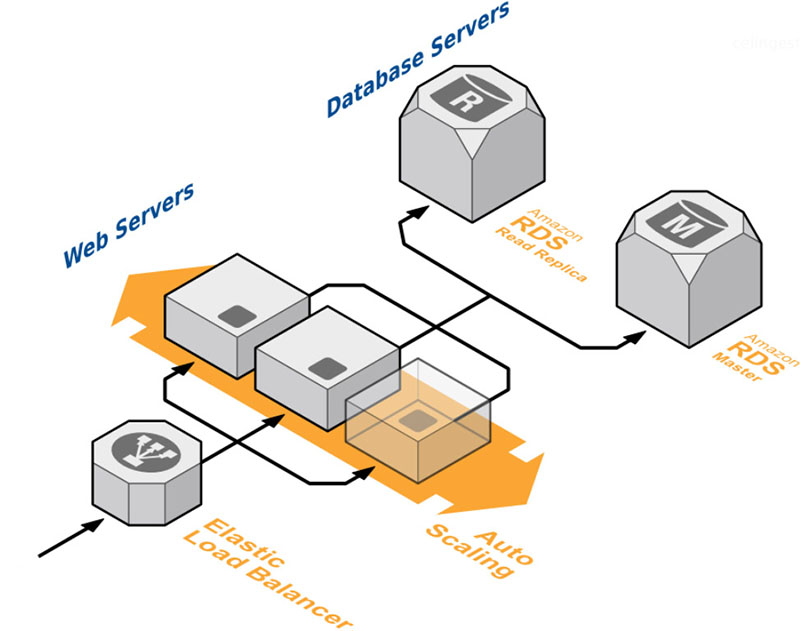
\includegraphics[width=\linewidth]{imgs/load_balancer.jpg}
	\caption{Esempio di Auto Scaling for AWS}
	\label{fig:autoscaleAWS}
\end{figure}
Uno servizio molto import di Amazon è \textbf{AutoScaling}(Fig \ref{fig:autoscaleAWS}). Per far funzionare AutoScaling è importante anche il \textbf{Elastic Load Balancer}, grazie al quale l'utente finale vedere solo un collegamento e Elastic Load Balancer pensa a distribuire le richiede alle nostre macchine. 
Le istanze EC2 possono essere categorizzate in auto scaling groups, di solito con un range tra un minimo e un massimo, se una nuova macchina entra in esecuzione oppure viene de-allocata il Load Balancer viene avvertito della modifica in modo che possa funzionare bene.
Gli Auto Scaling group sono istanze EC2 che condividono caratteristiche simili e devono essere fatte per scalare, e aggiunge automaticamente un nuovo nodo in base a policy definite dall'utente, programmazione oppure health checks e workload e la nuova istanza può venire anche da availability zone diverse della stessa regione.\\
Auto Scaling group contiene solo un launch configuration che descrive le istanze che devono far partire (contiene i parametri delle AMI), se si aggiorna il launch configuration questo affliggerà solo le nuove istanze, le vecchie istanze rimangono tali ma esse vengono terminate prima durante un scale in.\\
%\section{Lezione 5 - 16/10}
Attenzione una macchina può essere o spenta o terminata, nel caso viene terminata viene eliminata completamente e AutoScaling group termina una macchina.\\
L'ecosistema di Auto Scaling è composta da:
\begin{myitemize}
	\item Cloud Watch: Per monitorare le istanze EC2, le metriche più usate per il CloudWatch sono:
	\begin{myitemize}
		\item CPU usage
		\item Latenza
		\item Numero di Richieste
		\item Il numero di Host(macchine) in buona salute
		\item Il numero di macchine non in buona salute
	\end{myitemize}
	\item Elastic Load Balancer: Per distribuire il lavoro su un numero qualunque di istanze EC2 ed effettuare controlli periodici sulla salute del nodo (basandosi sul tempo di risposta) e in caso non siano in buona salute il load balancer smette di inviare a lui le richieste.
	\item Auto Scaling: Utilizza i dati collezionati dal CloudWatch per costruire sistemi che posso scalare (dentro o fuori) all'intero del range
\end{myitemize}
Il \textbf{Trigger} è un meccanismo di attivare una policy, in questo caso di aumentare o diminuire il numero dei nodi. Il trigger può essere attivato da un allarme cloud watch (configurato per guardare una metrica di cloud watch) oppure un auto scaling policy che descrive cosa fare in caso di un allarme. Quando si attiva il trigger lancia un processo chiamato Scaling activity che esegue la auto scaling policy.
Osservazione Auto Scaling supporta ma non necessita Elastic Load Balancer.
In generale almeno due trigger sono necessari, uno per Scale up e uno per Scale down, per mantenere un equilibrio desiderato.
Un allarme è una metrica e verifica se questa metrica supera un limite stabilito per un certo tempo.\\
Un'allarme è un'entità in grado di osservare con continuità una certa metrica e ci indica se tale metrica ha superato un certo valore prefissato per un certo tempo, per creare un allarme è necessario specificare:
\begin{myitemize}
	\item Metrica da osservare
	\item Il threshold della metrica
	\item Il numero di periodo di valutazione
\end{myitemize}
Gli stati in cui l'allarme si può trovare sono:
\begin{myitemize}
	\item Ok, tutto bene! Metrica è sotto il threshold.
	\item Alarm: Metrica è sopra il threshold, è necessaria un azione.
	\item Dati Insufficiente, metrica disponibile o non ci sono abbastanza dati.
\end{myitemize}
Se l'allarme cambia lo stato e vi rimane per un determinato periodo di valutazione, un'azione viene invocata in base alla policy.\\
I scenari automatici dell'auto scaling sono:
\begin{myitemize}
	\item Fleet Management: assicura il performance ottimale della macchina, controllando la salute dell'istanza con Health Check: se un'istanza dovesse terminare questa viene individuata e si fa partire un'altra macchina.
	\item Scheduled scaling: Azioni vengono eseguite in maniera programmata, quindi è una sorta di evento temporale per eventi ricorsivi o scheduled.
	\item Scaling Dinamico: In base all'allarme su una metrica c'è una politica che risponde all'allarme. L'azione può dipendere step-wise da gravità dell'allarme oppure facendo tracking di una certa metrica e aggiusto il sistema in modo da calmare l'allarme.
\end{myitemize}
La terminazione della macchina può essere fatta anche per un ribilanciamento delle macchine nelle availability zone, la precedenza dello spegnimento viene data in modo da bilanciare tra le zone seguito dal fatto di voler preservare le macchine con il launch configuration più recente seguito dalla macchina prossima allo scatto dell'ora (per il prezzo che si paga ogni ora).
Auto Scaling inizializza una nuova istanza prima di spegnerne una per non compromettere la disponibilità e le performance dell'applicazione.\\
Dopo che è iniziata la fase di Auto Scaling esiste un periodo di cooldown, in questo periodo nessun altra attività di scaling può iniziare.\\
I canditati per autoscaling sono:
\begin{myitemize}
	\item Web Tier - sistemi che forniscono servizi web
	\item Application Tier
	\item Load Balancing Tier - sistemi che gestiscono il carico
	\item Stateless Tier - sistemi sono prive di stato es. funzioni pure, sono prive di memoria e quindi da un punto di visto funzionale non cambia se faccio autoscaling o no.
\end{myitemize}
I candidati che non dovrebbero fare autoscaling:
\begin{myitemize}
	\item Database Relazionali
	\item Database non-relazionali
	\item Sistema di caching distribuito
	\item Elastic Search
	\item Sistemi con lo stato - es. Kafka, non avrebbe senso fare autoscaling automatico.
\end{myitemize}

\section{PaaS with Azure}

\end{document}
